\chapter{Group Actions}
A group action is a representation of the elements of a group as symmetries of a set. Many groups have a `natural' group action coming from their construction. For example, the dihedral group of order 6, $D_3$, acts on the vertices of an equilateral triangle naturally because the group is, by definition, given as a set of symmetries of the equilateral triangle. A group action of a group on a set is a generalization of this idea, which can be used to derive useful facts about the group and the set it acts on.

\section{Definition and Examples}
\begin{definition}\label{definition-group-action}
    Let $G$ be a group, $e$ be the identity in $G$, and $X$ be a set. A \textbf{group action of $G$ on $X$}\index{group action} is a function $\alpha: G \times X \to X$ satisfying the following axioms.
    \begin{itemize}
        \item \textbf{Identity}: $\alpha(e, x) = x$ for all $x \in X$.
        \item \textbf{Compatibility}: $\alpha(g, \alpha(h, x)) = \alpha(gh, x)$ for all $g, h \in G$ and $x \in X$.
    \end{itemize}
\end{definition}
\begin{remark}
    Some sources will use $f$ (e.g. \cite{brilliant_group-actions}) or $\phi$ (e.g. \cite{rowland_group-action}) as the group action.
\end{remark}
In this case, the group $G$ is called a \textbf{transformation group}\index{transformation group} and $X$ is called a \textbf{$G$-set}\index{$G$-set}.

\newpage

Often the function $\alpha(g, x)$ is often written as $g \cdot x$ instead. Note that, when mentioning the group action, we \textbf{will} write the dot in this book. With this notation, the axioms above become:
\begin{itemize}
    \item $e \cdot x = x$ for all $x \in X$; and
    \item $g \cdot (h \cdot x) = (gh) \cdot x$ for all $g, h \in G$ and $x \in X$.
\end{itemize}

\begin{example}
    Consider the group $G = \Sn{n}$ and the set $X = \{1, 2, 3, \dots, n\}$. Then $G$ acts naturally on $X$ by the function $\alpha$, where $\alpha(g, x) = g(x)$. That is, $g \cdot x = g(x)$ in this case. We note that the axioms are satisfied.
    \begin{itemize}
        \item \textbf{Identity}: $\id \cdot x = \id(x) = x$.
        \item \textbf{Compatibility}: $g \cdot (h \cdot x) = g(h(x)) = (g \circ h)(x) = (gh) \cdot x$.
    \end{itemize}
\end{example}

\begin{example}
    Let $G$ be any group and the function $\alpha: G\times G \to G$ be defined such that $\alpha(g, x) = gx$. We show that $\alpha$ is a group action of $G$ on $G$.
    \begin{itemize}
        \item \textbf{Identity}: $e\cdot x = ex = x$.
        \item \textbf{Compatibility}: $g \cdot (h\cdot x) = g \cdot (hx) = ghx = (gh)x = (gh) \cdot x$.
    \end{itemize}
\end{example}

\begin{exercise}\label{exercise-conjugacy-is-group-action}
    Let $G$ be a group and the function $\alpha: G\times G \to G$ be defined such that $\alpha(g, x) = gxg^{-1}$. Show that $\alpha$ is a group action of $G$ on $G$.
\end{exercise}

We note that there is an equivalent definition of a group action of $G$ on $X$.
\begin{definition}\label{definition-group-action-alt}\index{group action}
    Let $G$ be a group and $X$ be a set. Then a group action of $G$ on $X$ is a homomorphism $\phi: G\to \Sym{X}$.
\end{definition}
\begin{theorem}\label{thrm-group-action-definition-equivalence}
    \myref{definition-group-action} and \myref{definition-group-action-alt} are equivalent.
\end{theorem}
\begin{proof}
    We first work forwards, assuming \myref{definition-group-action} is true and proving \myref{definition-group-action-alt} is true as well.
    
    Assume $\alpha: G \times X \to X$ is a group action. Define $\psi: G \to \Sym{X}$ by $g \mapsto f_g$ where the map $f_g: X \to X, x \mapsto \alpha(g, x)$. We show that $f_g$ is a bijection.
    \begin{itemize}
        \item \textbf{Injective}: Suppose there exists $x, y \in X$ such that $f_g(x) = f_g(y)$. Then,
        \begin{align*}
            x &= \alpha(e, x)\\
            &= \alpha(g^{-1}g, x)\\
            &= \alpha(g^{-1}, \alpha(g, x))\\
            &= \alpha(g^{-1}, f_g(x))\\
            &= \alpha(g^{-1}, f_g(y))\\
            &= \alpha(g^{-1}, \alpha(g, y))\\
            &= \alpha(g^{-1}g, y)\\
            &= \alpha(e, y)\\
            &= y
        \end{align*}
        so $f_g$ is injective.
        \item \textbf{Surjective}: Suppose $y \in X$. We note that $\alpha(g^{-1}, y) \in X$ by definition of $\alpha$. Hence observe that $f_g(\alpha(g^{-1}, y)) = \alpha(g, \alpha(g^{-1}, y)) = y$, which means that any element $y \in X$ has a pre-image in $X$. This shows that $f_g$ is surjective.
    \end{itemize}
    Hence $f_g$ is a bijection from $X$ to $X$, which means $f_g \in \Sym{X}$. We just need to show that $\psi$ is a homomorphism. Take $x \in X$, and let $g, h \in G$. Then
    \begin{align*}
        (\psi(gh))(x) &= f_{gh}(x)\\
        &= \alpha(gh, x)\\
        &= \alpha(g, \alpha(h, x))\\
        &= \alpha(g, f_h(x))\\
        &= f_g(f_h(x))\\
        &= (f_g \circ f_h)(x)\\
        &= (\psi(g)\psi(h))(x)
    \end{align*}
    for any $x \in X$, which means $\psi(gh) = \psi(g)\psi(h)$. Hence $\phi$ is indeed a homomorphism, satisfying \myref{definition-group-action-alt}.

    We now work in the reverse direction, assuming that \myref{definition-group-action-alt} holds and proving \myref{definition-group-action} holds as well.
    
    Suppose $\phi: G \to \Sym{X}$ is a group homomorphism. We define $\beta: G \times X \to X$ where $\beta(g, x) = (\phi(g))(x)$. We verify \myref{definition-group-action} holds for $\beta$.
    \begin{itemize}
        \item \textbf{Identity}: Since $\phi$ is a homomorphism, it must map the identity in $G$ to the identity in $\Sym{X}$, which is $\id$. Hence, $\beta(e, x) = (\phi(e))(x) = \id(x) = x$.
        \item \textbf{Compatibility}: Let $g, h \in G$ and $x \in X$. Then
        \begin{align*}
            \beta(g, \alpha(h, x)) &= \beta(g, (\phi(h))(x))\\
            &= (\phi(g))((\phi(h))(x))\\
            &= (\phi(g) \circ \phi(h))(x)\\
            &= (\phi(gh))(x)\\
            &= \beta(gh, x).
        \end{align*}
    \end{itemize}
    Therefore \myref{definition-group-action} holds for $\beta$.

    The final thing to prove equivalence of the definitions is to show that the above processes are `inverses' of each other. That is, we want to show that
    \begin{itemize}
        \item if we start with $\alpha$, derive $\psi$ based on $\alpha$, and then derive $\beta$ based off $\psi$, then $\alpha = \beta$; and
        \item if we start with $\phi$, derive $\beta$, and then derive $\psi$ based off $\beta$, then $\phi = \psi$.
    \end{itemize}

    Suppose we have an $\alpha$ that is used to derive $\psi$ which is in turn used to derive $\beta$. Then the above processes yields
    \[
        \psi(g) = f_g \text{ and } \beta(g, x) = (\psi(g))(x)
    \]
    where $f_g(x) = \alpha(g, x)$. Hence $\alpha(g, x) = f_g(x) = (\psi(g))(x) = \beta(g, x)$ for any $g \in G$ and $x \in X$. Hence $\alpha = \beta$.

    Now suppose we have a $\phi$ that is used to derive $\beta$ which is in turn used to derive $\psi$. Then the above processes yields
    \[
        \beta(g, x) = (\phi(g))(x) \text{ and } \psi(g) = f_g
    \]
    where $f_g(x) = \beta(g, x)$ in this case. Hence $(\phi(g))(x) = \beta(g, x) = f_g(x) = (\psi(g))(x)$ for any $g \in G$ and $x \in X$. Hence $\phi = \psi$.

    Therefore, this shows that the maps $\alpha \mapsto \phi$ and $\phi \mapsto \alpha$ are inverses of each other, so we have a one-to-one correspondence between \myref{definition-group-action} and \myref{definition-group-action-alt}.
\end{proof}
\begin{remark}
    What this theorem also shows is that a group action $\alpha$ induces a group homomorphism $\phi: G \to \Sym{X}$. In addition, if $X$ is finite with $n$ elements, a homomorphism $\phi: G \to \Sn{n}$ exists (since $\Sym{X} \cong \Sn{n}$ by \myref{corollary-symmetric-group-of-finite-order}).
\end{remark}

\section{Fixed Points, Stabilizers, and Orbits}
We first look at the definition of a \textbf{fixed point} in relation to group actions.

\begin{definition}
    Let $G$ be a group acting on a set $X$. A \textbf{fixed point of $g \in G$}\index{group action!fixed point} is an element $x \in X$ such that $g\cdot x = x$.
\end{definition}

\begin{example}
    Consider the group $G = \{e, g\}$ (where $g^2 = e$) and the set $X = \mathbb{Z}$. Let $G$ act on $X$ by the formulae $e\cdot x = x$ and $g\cdot x = -x$. We find the fixed points of every element in $G$.
    \begin{itemize}
        \item For $e$, every element in $X$ is a fixed point of it.
        \item For any other element $g$, 0 is the only fixed point since $g\cdot 0 = -0 = 0$.
    \end{itemize}
\end{example}

\begin{exercise}
    Let $X = \{1, 2, 3\}$, and let $\Sn{3}$ act on $X$. What are the fixed point(s) of each of the 6 actions in $\Sn{3}$?
\end{exercise}

With an understanding of fixed points, we can now look at the \textbf{stabilizer} of an element in $X$.

\begin{definition}
    Let $G$ be a group acting on a set $X$, and let $x \in X$. The \textbf{stabilizer of $x$ by $G$}\index{group action!stabilizer}, denoted $\Stab{G}{x}$, is the set of $g \in G$ such that $x$ is a fixed point of $g$.
\end{definition}
\begin{remark}
    Some authors will denote the stabilizer of $x$ by $G$ by $G_x$ (e.g. \cite{clark_1984, humphreys_1996, brilliant_group-actions}).
\end{remark}

\begin{example}
    Consider again the group $G = \{e, g\}$ and the set $X = \mathbb{Z}$ with relations defined in the previous example.
    \begin{itemize}
        \item Let's find the stabilizer of 0, $\Stab{G}{0}$. Thus we are finding the set of $f \in G$ such that 0 is a fixed point of $f$. Note that $g \cdot 0 = -0 = 0$ for any $g \in G$ so the entirety of $G$ forms the stabilizer of 0, i.e. $\Stab{G}{0} = G$.
        \item Now consider the stabilizer of any non-zero integer in $X$, say $x \in X$. We are finding the set of $f \in G$ such that $x$ is a fixed point of $f$. Note that for any non-identity $g \in G$, we have $g \cdot x = -x \neq x$. Thus, the only element in $G$ that makes $x$ a fixed point is $e$, i.e. $\Stab{G}{x} = \{e\}$ if $x \neq 0$.
    \end{itemize}
    To summarise, $\Stab{G}{0} = G$ and $\Stab{G}{x} = \{e\}$ if $x \neq 0$.
\end{example}

\begin{exercise}
    Let $X = \{1, 2, 3\}$, and let $\Sn{3}$ act on $X$. What are the stabilizers of each of the 3 elements in $X$?
\end{exercise}

What you might notice from the above example and exercise is that the stabilizers are sub\textit{sets} of the original group $G$. In fact, we will prove that the stabilizer is a sub\textit{group} of $G$.

\begin{lemma}\label{lemma-stabilizer-is-subgroup}
    Let $G$ be a group that acts on a set $X$. Then for any $x \in X$, $\Stab{G}{x} \leq G$.
\end{lemma}
\begin{proof}
    We consider the subgroup test.

    We note $e \in G$. From the group action axiom of \textbf{Identity}, we know that $e \cdot x = x$. Thus, for any element $x$, we have $e \in \Stab{G}{x}$. Hence $\Stab{G}{x}$ is non-empty.

    Now consider $g, h \in \Stab{G}{x}$. This means that $g\cdot x = x$ and $h \cdot x = x$. We note that
    \begin{align*}
        h^{-1} \cdot x &= h^{-1} \cdot (h \cdot x) & (\text{as } h \in \Stab{G}{x}, \text{ so } h\cdot x = x)\\
        &= (h^{-1}h) \cdot x & (\text{\textbf{Compatibility} Axiom})\\
        &= e \cdot x\\
        &= x
    \end{align*}
    so $h^{-1} \in \Stab{G}{x}$. Now consider $gh^{-1}$.
    \begin{align*}
        (gh^{-1}) \cdot x &= g \cdot (h^{-1} \cdot x) & (\text{\textbf{Compatibility} Axiom})\\
        &= g \cdot x & (h^{-1} \in \Stab{G}{x})\\
        &= x & (g \in \Stab{G}{x})
    \end{align*}
    which means that $gh^{-1} \in \Stab{G}{x}$.

    Thus, by subgroup test, $\Stab{G}{x} \leq G$ for any $x \in X$.
\end{proof}

\begin{exercise}\label{exercise-group-action-outputs-equal-iff-gh^-1-in-stabilizer}
    Let $G$ be a group that acts on a set $X$. Prove that $g \cdot x = h \cdot x$ if and only if $g^{-1}h \in \Stab{G}{x}$.
\end{exercise}

We now look at the definition of the \textbf{orbit} of an element.
\begin{definition}
    Let $G$ be a group acting on a set $X$, and suppose $x \in X$. The \textbf{orbit of $x$ in $G$}\index{group action!orbit}, denoted $\Orb{G}{x}$, is the set of elements $y \in X$ such that $g \cdot x = y$ for some $g \in G$.
\end{definition}
\begin{remark}
    Some authors will denote the orbit of $x$ in $G$ by $G \cdot x$ (e.g. \cite{clark_1984}) or simply by $Gx$ (e.g. \cite{milne_2021}).
\end{remark}

\begin{example}
    Consider again the group $G = \{e, g\}$ with $g^2 = e$ and let $G$ act on the set $X = \mathbb{Z}$ such that $e \cdot x = x$ and $g \cdot x = -x$. Note that the orbit for any non-zero element $x \in X$ is the set $\{x, -x\}$, while the orbit for 0 is $\{0\}$ itself.
\end{example}

We say that a group action is \textbf{transitive}\index{group action!transitive} if and only if it has one orbit. That is to say, the group action is transitive if there exists $x \in X$ such that $\Orb{G}{x} = X$.

\begin{exercise}
    Let $G$ be a group that acts on a non-empty set $X$. Show that if the group action is transitive if and only if $\Orb{G}{x} = X$ for \textbf{all} $x \in X$.
\end{exercise}

\begin{exercise}\label{exercise-distinct-orbits-partition-set}
    Let $G$ be a group that acts on a non-empty set $X$. Prove that
    \begin{partquestions}{\alph*}
        \item every element in $X$ is in some orbit; and
        \item if $\Orb{G}{x_1} \cap \Orb{G}{x_2} \neq \emptyset$ where $x_1, x_2 \in X$, then $\Orb{G}{x_1} = \Orb{G}{x_2}$.
    \end{partquestions}
    \textit{(That is, prove that distinct orbits partition $X$.)}
\end{exercise}

\section{The Orbit-Stabilizer Theorem}
There is a natural relationship between orbits and stabilizers of a group action. We give the intuition of the theorem before stating it formally.

Let's think about the symmetric group of a cube (call it $G$) and suppose $G$ acts on the set of faces of the cube, $F$. How many elements are there in $G$? We could do the following:
\begin{enumerate}
    \item Fix one face (say the top face). There are 4 ways to move the cube because you can only rotate the cube now. These are the `stabilizers'.
    \item Now there are 6 choices for which face to be fixed. This is the `orbit'.
\end{enumerate}
Thus, the total number of elements in the symmetric group of a cube is 24, i.e. $|G| = 24$. Generally, the number of elements of a transformation group $G$ is the product of the orders of the stabilizer and orbit of an element $x$ in the $G$-set.

Formally, this is captured in the \textbf{Orbit-Stabilizer Theorem}.
\begin{theorem}[Orbit-Stabilizer]\label{thrm-orbit-stabilizer}\index{Orbit-Stabilizer Theorem}
    Let $G$ be a group that acts on a finite set $X$. Let $x \in X$. Then
    \[
        |G| = |\Stab{G}{x}| \times |\Orb{G}{x}|.
    \]
    In other words, the order of the group $G$ is the product of the order of the stabilizer of $x$ and the number of elements in the orbit of $x$.
\end{theorem}

\begin{proof}[Proof (see {\cite[Theorem 10.16]{humphreys_1996}})]
    We consider the map $f_x: G/\Stab{G}{x} \to \Orb{G}{x}$ given by $g\Stab{G}{x} \mapsto g \cdot x$ (note that $f_x$ is \textit{not} a homomorphism as $\Orb{G}{x}$ is not a group). We prove that $f_x$ is a well-defined bijection.
    \begin{itemize}
        \item \textbf{Well-defined}: Suppose we have $g, h \in G$ such that we have $g\Stab{G}{x} = h\Stab{G}{x}$. By Coset Equality (\myref{lemma-coset-equality}), this means that $g^{-1}h \in \Stab{G}{x}$. Furthermore, by \myref{exercise-group-action-outputs-equal-iff-gh^-1-in-stabilizer}, this means that $g\cdot x = h\cdot x$. Hence, $f_x(g\Stab{G}{x}) = f_x(h\Stab{G}{x})$, meaning that $f_x$ is well-defined.
        \item \textbf{Injective}: Suppose we have $g, h \in G$ such that we have $f_x(g\Stab{G}{x}) = f_x(h\Stab{G}{x})$, meaning $g\cdot x = h\cdot x$, so $g^{-1}h \in \Stab{G}{x}$ by \myref{exercise-group-action-outputs-equal-iff-gh^-1-in-stabilizer}. Hence $g\Stab{G}{x} = h\Stab{G}{x}$ by Coset Equality (\myref{lemma-coset-equality}), meaning $f_x$ is injective.
        \item \textbf{Surjective}: Suppose $y \in \Orb{G}{x}$. This means that there exists $g \in G$ such that $g\cdot x = y$. Note $f_x(g\Stab{G}{x}) = g\cdot x = y$ by definition of $f_x$. Hence, the pre-image of $y$ is $g\Stab{G}{x}$, meaning that $f_x$ is surjective.
    \end{itemize}
    Hence $f_x$ is a bijection from $G/\Stab{G}{x}$ to $\Orb{G}{x}$. Therefore we must have $|\Orb{G}{x}| = |G/\Stab{G}{x}| = \frac{|G|}{|\Stab{G}{x}|}$ by Lagrange's Theorem (\myref{thrm-lagrange}). This quickly implies $|G| = |\Stab{G}{x}|\times|\Orb{G}{x}|$.
\end{proof}

\begin{exercise}
    Let $G = \Sn{n}$ be a transformation group and $X = \{1, 2, 3, \dots, n\}$ be a $G$-set.
    \begin{partquestions}{\roman*}
        \item Show that the group action is transitive.
        \item Find the order of the stabilizer of $x \in X$ by $G$.
    \end{partquestions}
\end{exercise}

\section{Burnside's Lemma}
Burnside's lemma gives a way to count the number of orbits of a finite set acted on by a finite group. Before we get into it, we look at the \textbf{set of orbits of $X$}.

\begin{definition}
    The \textbf{set of orbits}\index{set of orbits} acted upon by the group $G$ on a set $X$ is the set
    \[
        X / G = \{\Orb{G}{x} \vert x \in X\}.
    \]
    That is, $X/G$ is the set of distinct orbits over all elements of $X$.
\end{definition}
\begin{remark}
    The number of distinct orbits is given by the number of elements of the set $X/G$, i.e. $|X/G|$.
\end{remark}

\newpage

We are now ready to introduce Burnside's lemma.
\begin{lemma}[Burnside]\label{lemma-burnside}\index{Burnside's Lemma}
    Let $G$ be a finite group acting on a set $X$. Let $\Fix{X}{g}$ denote the set of all elements in $X$ which is fixed by $g$, that is,
    \[
        \Fix{X}{g} = \{x \in X \vert g\cdot x = x\}.
    \]
    Then
    \[
        |X/G| = \frac{1}{|G|}\sum_{g\in G} |\Fix{X}{g}|.
    \]
\end{lemma}
In other words, Burnside's lemma tells us that the number of orbits is the average number of fixed elements for each $g \in G$.
\begin{proof}[Proof (see \cite{proofwiki_burnsides-lemma})]
    We start by noting that
    \begin{align*}
        \sum_{g\in G} |\Fix{X}{g}| &= \sum_{g\in G} |\{x \in X \vertalt g\cdot x = x\}|\\
        &= |\{(g, x) \vert g \in G,\; x \in X \text{ such that } g\cdot x = x\}|\\
        &= \sum_{x\in X} |\{g \in G \vertalt g\cdot x = x\}|\\
        &= \sum_{x\in X} |\Stab{G}{x}|.
    \end{align*}
    One sees that $|\Stab{G}{x}| = \frac{|G|}{|\Orb{G}{x}|}$ by the Orbit-Stabilizer theorem (\myref{thrm-orbit-stabilizer}). Thus,
    \begin{align*}
        \sum_{x\in X} |\Stab{G}{x}| &= \sum_{x\in X} \frac{|G|}{|\Orb{G}{x}|}\\
        &= |G|\sum_{x\in X} \frac{1}{|\Orb{G}{x}|}.
    \end{align*}
    Notice that $X$ is the disjoint union of all orbits in $X/G$ (\myref{exercise-distinct-orbits-partition-set}), which means the sum over $X$ may be broken up into separate sums over each individual orbit. Thus,
    \begin{align*}
        \sum_{x\in X} \frac{1}{|\Orb{G}{x}|} &= \sum_{\Orb{G}{x} \in X/G}\left(\sum_{x \in \Orb{G}{x}} \frac{1}{|\Orb{G}{x}|}\right)\\
        &= \sum_{\Orb{G}{x} \in X/G} 1\\
        &= |X/G|.
    \end{align*}
    Putting everything together,
    \[
        \sum_{g\in G} |\Fix{X}{g}| = |G||X/G|
    \]
    which the result follows immediately.
\end{proof}

\begin{example}
    We find the number of distinct colourings of the corners on a square with $n$ colours (up to rotation) using by Burnside's lemma.

    \begin{figure}[h]
	    \centering
	    \fbox{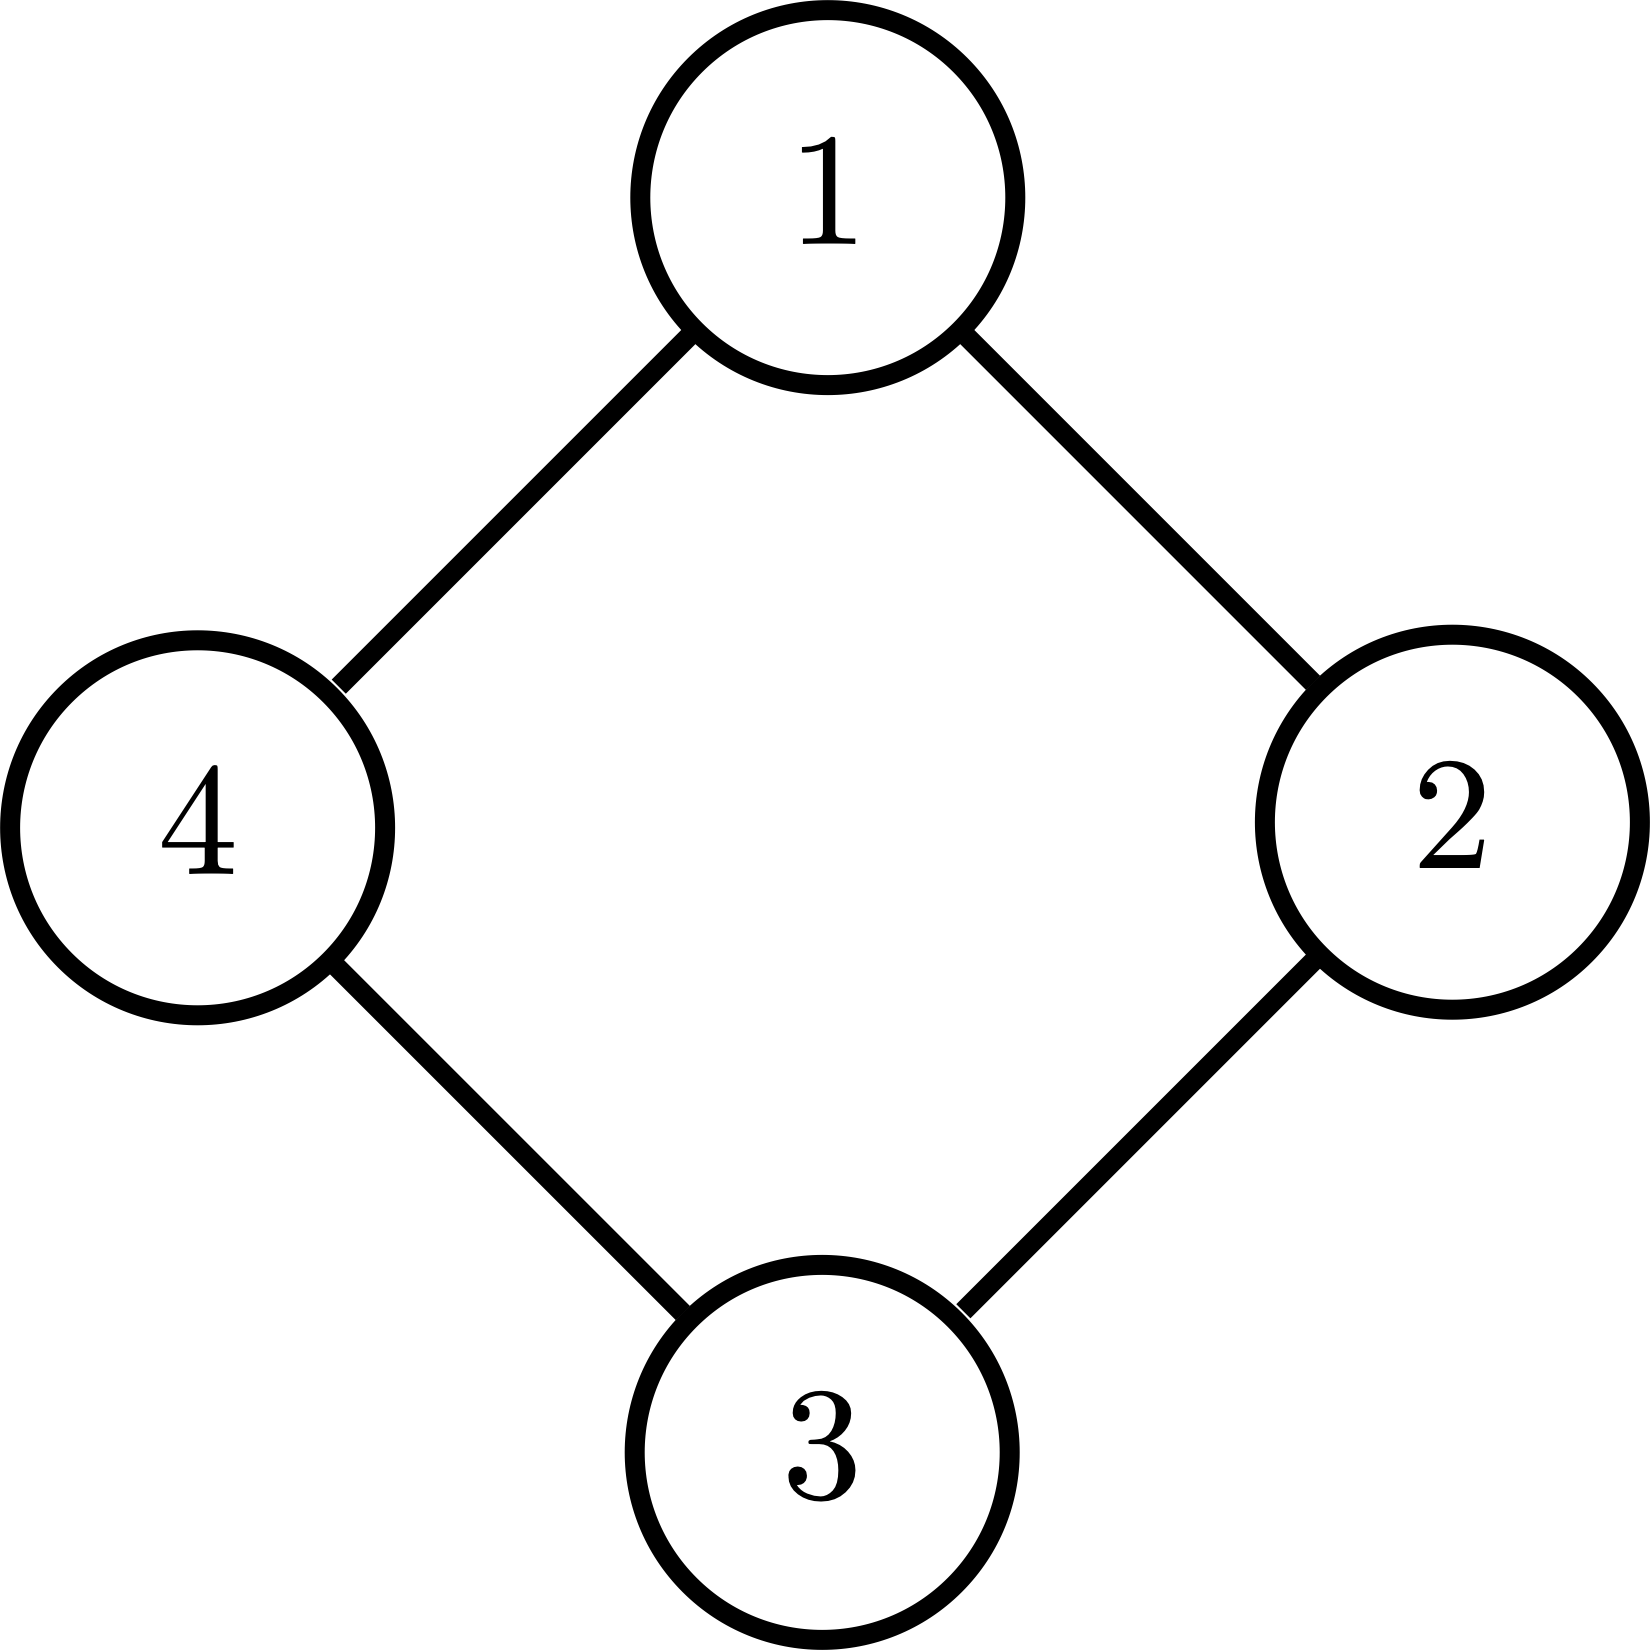
\includegraphics[width=3.5cm]{chapter9/Labelled Square.png}}
	    \caption{Square With Labelled Corners}
	\end{figure}

    Let $X$ denote the set of colourings of the corners of the square, and let $G$ denote the rotation group acting on $X$. Then two elements of $X$ belong to the same orbit precisely when one is simply a rotation of the other. We note that $G$ consists of four $90^\circ$ rotations, so $G$ is generated by the $90^\circ$ rotation action, meaning $G \cong \Cn{4}$.
    \begin{enumerate}
        \item Rotating the square $0^\circ$ does not change the colourings at all, which means that the number of fixed points is the total number of possible colourings, which is $n^4$.
        \item Rotating the square $90^\circ$ results in all points affecting one another, so the only fixed points would be colourings of all the same color. Since there are $n$ different colours, thus the number of fixed points is $n$.
        \item Rotating the square $180^\circ$ swaps two pairs of vertices that are across from each other. Thus, a fixed point will occur if the two pairs have the same colour. Hence, there are $n^2$ fixed points.
        \item Finally, rotating the square $270^\circ$ is similar to rotating $90^\circ$, so there are $n$ fixed points.
    \end{enumerate}
    There are 4 elements in $G$, so $|G| = 4$. By Burnside's lemma (\myref{lemma-burnside}),
    \[
        |X/G| = \frac{1}{|G|}\sum_{g\in G} |\Fix{X}{g}| = \frac14 (n^4 + n + n^2 + n),
    \]
    i.e., the number of distinct possible colourings of the corners on a square with $n$ colours (up to rotation) is $\frac n4 (n^3 + n + 2)$.
\end{example}

\newpage

\section{Conjugacy Classes}
Before we look at the most important part of this chapter, the class equation, we look at the idea of conjugacy as a group action.
\begin{definition}
    Let $G$ be a group, and suppose $a, b \in G$. Then we say that $b$ is a \textbf{conjugate}\index{conjugate} of $a$ if there is an element $g \in G$ such that $b = gag^{-1}$ (or, alternatively, $a=g^{-1}bg$).
\end{definition}
We can frame this idea in terms of group actions.

Consider the map $\alpha: G\times G\to G$ such that $\alpha(g, x) = gxg^{-1}$. We showed that $\alpha$ is a group action in \myref{exercise-conjugacy-is-group-action}. Let's look at the orbit and stabilizer of an arbitrary element $x \in G$ under this group action.
\begin{itemize}
    \item For the orbits, we are to find a $y \in G$ such that there exists a $g \in G$ where $gxg^{-1} = y$. Hence, the orbit of $x$ under this group action are the conjugates of $x$.
    \item For the stabilizer, we are to find elements $g \in G$ such that $gxg^{-1} = x$. Hence any such element satisfies $gx = xg$. Therefore, $g \in \C{G}{x}$ where $\C{G}{x}$ is the centralizer of $x$ (recall how it is defined in \myref{example-centralizer-of-a-subset}).
\end{itemize}

Hence, under the action of conjugation,
\begin{itemize}
    \item $\Orb{G}{x} = $ Conjugates of $x$; and
    \item $\Stab{G}{x} = \C{G}{x}$.
\end{itemize}

\newpage

We can now look at conjugacy classes.
\begin{definition}
    Let $G$ be a group and take $x \in G$. The \textbf{conjugacy class of $x$}\index{conjugacy class} is the set
    \[
        \Cl{x} = \{gxg^{-1} \vert g \in G\}.
    \]
    In other words, the set $\Cl{x}$ is a subset of $G$ where all elements inside it are conjugates of each other.
\end{definition}
\begin{remark}
    We omit having the subscript of $G$ for the conjugacy class since $x \in G$. Also, under the group action of conjugation, $\Orb{G}{x} = \Cl{x}$.
\end{remark}

\begin{example}\label{example-conjugacy-classes-of-Sn3}
    We look at distinct conjugacy classes of $\Sn{3}$.
    \begin{itemize}
        \item The first is the conjugacy class of the identity, $\id$.
        \[
            \Cl{\id} = \{g\circ\id\circ g^{-1} \vert g \in G \} = \{\id\}.
        \]
        Thus the conjugacy class of the identity consists of only the identity.
        \item The second is the conjugacy class of transpositions. Let $\tau = \begin{pmatrix}a & b\end{pmatrix}$ be a transposition in $\Sn{3}$. Then
        \[
            \Cl{\tau} = \{g\circ\tau\circ g^{-1} \vert g \in G\}.
        \]
        Running through all 6 elements of $\Sn{3}$ reveals that $\Cl{\tau}$ is the set of all transpositions, i.e. the conjugacy class of transpositions is the set of transpositions.
        \item The third is the conjugacy class of 3-cycles. Let $\sigma = \begin{pmatrix}a & b & c\end{pmatrix}$ be a 3-cycle in $\Sn{3}$. One can see that $\Cl{\sigma}$ is the set of all 3-cycles.
    \end{itemize}
\end{example}

\begin{exercise}\label{exercise-order-of-conjugacy-class}
    Let $G$ be a group and $x \in G$. Prove that
    \[
        |\Cl{x}| = [G : \C{G}{x}].
    \]
\end{exercise}

\section{The Class Equation}
The example of the previous section illustrates that the sum of the sizes of the conjugacy classes must be equal to the size of the group. This fact, along with the Orbit-Stabilizer theorem (\myref{thrm-orbit-stabilizer}), can be used to derive an important equation known as \textbf{the class equation}.

Before we state and prove the class equation, we recall the center of a group as introduced in \myref{example-center-of-group}.
\begin{quote}
    The center of a group $G$ is the normal subgroup
    \[
        \Z{G} = \{z \in G \vert gz = zg \text{ for all } g \in G\}.
    \]
    In other words, $\Z{G} = \{z \in G \vert z = gzg^{-1} \; \forall g \in G\}$.
\end{quote}

We now state and prove the class equation.
\begin{theorem}[Class Equation]\label{thrm-class-equation}
    Let $G$ be a finite group. Suppose $G$ has $k$ conjugacy classes, with $l$ of them having more than 1 element. Suppose $g_1, g_2, \dots, g_l$ are representatives of the conjugacy classes with more than 1 element. Then
    \[
        |G| = |\Z{G}| + \sum_{i=1}^l [G : \C{G}{g_i}],
    \]
    which is known as \textbf{the class equation}\index{Class Equation}.
\end{theorem}

\begin{proof}
    We know by \myref{exercise-distinct-orbits-partition-set} that distinct orbits partitions the set that the group is acting on. Hence, using the group action of conjugation, orbits under conjugation partition $G$. So
    \[
        G = \bigcup_{i=1}^k \Orb{G}{\hat{g_i}} = \bigcup_{i=1}^k \Cl{\hat{g_i}}
    \]
    where $\hat{g_i}$'s are representatives of the $k$ conjugacy classes (including those with only 1 element).

    Suppose now that an element $x$ is in a conjugacy class with one element. This means that $gxg^{-1} = x$ for all $g \in G$, so $x \in \Z{G}$.

    Therefore, one concludes that
    \[
        G = \left(\Z{G}\right) \cup \left(\bigcup_{i=1}^l \Cl{g_i}\right).
    \]
    Since this is a disjoint union, hence
    \[
        |G| = |\Z{G}| + \sum_{i=1}^l |\Cl{g_i}|.
    \]

    Finally, by \myref{exercise-order-of-conjugacy-class}, $|\Cl{g_i}| = [G : \C{G}{g_i}]$, which means that
    \[
        |G| = |\Z{G}| + \sum_{i=1}^l [G:\C{G}{g_i}]
    \]
    proving the theorem.
\end{proof}

We look at one application of the class equation. Before that, we introduce \textbf{$p$-groups}.
\begin{definition}
    A \textbf{$p$-group}\index{$p$-group} $G$ is a finite group with order $p^n$ where $p$ is prime and $n$ is a non-negative integer.
\end{definition}
An immediate consequence of this is that every element must have an order that is a power of $p$, i.e. for any element $x \in G$, $|x| = p^k$ where $0 \leq k \leq n$.

\begin{example}\label{example-group-with-prime-power-order-has-non-trivial-center}
    Let $G$ be a finite $p$-group, meaning $|G| = p^n$. We will show that $G$ has a non-trivial center using the class equation.

    Recall that $|\Cl{x}| = \frac{|G|}{|\C{G}{x}|}$ by \myref{exercise-order-of-conjugacy-class}. Hence, the order of the group must divide the order of any conjugacy class, i.e. $\frac{|G|}{|\C{G}{x}|} \vert |G|$. Since $|G| = p^n$, it follows that $|\Cl{x}| = p^k$ for some $1 \leq k \leq n$ (assuming $x \notin \Z{G}$).

    If $g_1, g_2, \dots, g_l$ are representatives from the conjugacy classes with more than 1 element, then this means that
    \[
        p^n = |G| = |\Z{G}| + \sum_{i=1}^l |\Cl{g_i}| = |\Z{G}| + \sum_{i=1}^l p^{k_i}
    \]
    where $1 \leq k_1, k_2, \dots, k_l < n$. From this, we conclude that $p$ must divide $|\Z{G}|$, meaning $|\Z{G}| > 1$.
\end{example}
\begin{example}
    We look at the class equation of the symmetric group of degree 3, $\Sn{3}$.

    Recall from \myref{example-conjugacy-classes-of-Sn3} that $\Sn{3}$ has the conjugacy classes
    \begin{align*}
        &\Cl{\id} = \{\id\}\\
        &\Cl{\tau} = \{\begin{pmatrix}1 & 2\end{pmatrix}, \begin{pmatrix}1 & 3\end{pmatrix}, \begin{pmatrix}2 & 3\end{pmatrix}\}\\
        &\Cl{\sigma} = \{\begin{pmatrix}1 & 2 & 3\end{pmatrix}, \begin{pmatrix}1 & 3 & 2\end{pmatrix}\}
    \end{align*}
    where $\tau$ is a 2-cycle (transposition) and $\sigma$ is a 3-cycle. Thus, the class equation of $\Sn{3}$ is
    \[
        6 = 1 + 2 + 3
    \]
    where $|\Z{\Sn{3}}| = |\{e\}| = 1$.  
\end{example}

\begin{exercise}
    The Cayley table of $D_3$ is in \myref{example-presentation-of-D3}.
    \begin{partquestions}{\alph*}
        \item Find $\Z{D_3}$, the center of $D_3$.
        \item For each conjugacy class of $D_3$ with more than 1 element, find a representative.
        \item Find the class equation of $D_3$.
    \end{partquestions}
\end{exercise}

\section{Cauchy's Theorem}
To end this chapter, we prove \textbf{Cauchy's Group Theorem}.
\begin{theorem}[Cauchy]\label{thrm-cauchy}\index{Cauchy's Theorem}
    Let $G$ be a finite group such that $|G| = np$ where $p$ is a prime and $n$ is a positive integer. Then $G$ contains an element of order $p$.
\end{theorem}
\begin{proof}
    We proceed with strong induction on $n$.

    For the case where $n = 1$, $|G| = p$. Then by \myref{exercise-prime-order-element}, every element of the group has order $p$, proving the base case.

    We now assume that the statement holds for all $n \leq k$ for some positive integer $k$. We need to prove the case for $k+1$, that is, a group $G$ with order $(k+1)p$ has an element of order $p$. We split the proof into two cases.

    The first case is when $G$ is abelian. Take any non-identity element $x \in G$, and let $H = \langle x \rangle \leq G$.
    \begin{itemize}
        \item If $p$ divides $|H|$, say $|H| = mp$ where $m$ is a positive integer, then $x^m$ is an element of order $p$ (since $\left(x^m\right)^p = x^{|H|} = e$). Hence we find an element with order $p$.
        \item If $p$ does not divide $|H|$, then $p$ must divide $[G:H] = |G/H| = \frac{|G|}{|H|}$ since $p$ divides $|G| = kp$. Note that $H \unlhd G$ since $G$ is abelian (\myref{prop-subgroup-of-abelian-group-is-normal}), so $G/H$ is a group. Letting $m = |x|$ we see
        \[
            (xH)^m = (x^m)H = eH = H \in G/H.
        \]
        Thus, $m$ is a multiple of $|G/H|$ (\myref{corollary-order-of-group-multiple-of-order-of-element}) which is in turn a multiple of $p$. Hence $p$ divides $m$, so $\frac mp$ is an integer and therefore $x^{\frac mp}$ is an element with order $p$ (since $\left(x^{\frac mp}\right)^p = x^m = e$).
    \end{itemize}
    Therefore, for the abelian case, there exists an element with order equal to $p$.

    We now consider the case when $G$ is non-abelian. Seeking a contradiction, assume $G$ does not have an element of order $p$. Let $H < G$, so $H$ has no element with order $p$. Therefore the contrapositive of the induction hypothesis means that $|H|$ is not a multiple of $p$. Note that Lagrange's Theorem (\myref{thrm-lagrange}) further gives that $|G| = [G:H]|H|$. Since $|H|$ is not divisible by $p$ and $|G|$ is divisible by $p$, we conclude that $p$ divides $[G:H]$ for every proper subgroup $H$.

    Since $G$ is non-abelian, thus $G \neq \Z{G}$ meaning that there exists at least one conjugacy class with more than 1 element. Suppose there are $l$ such classes, and let them be represented by the elements $g_1, g_2, \dots, g_l$. By the class equation (\myref{thrm-class-equation}),
    \[
        |G| = |\Z{G}| + \sum_{i=1}^l [G:\C{G}{g_i}].
    \]
    Note that $|\Cl{g_i}| = [G:\C{G}{g_i}] = \frac{|G|}{|\C{G}{g_i}|} > 1$, which means that $|G| > |\C{G}{g_i}|$. Thus $\C{G}{g_i} \neq G$ for all $i$. Recall that $\C{G}{g_i}$ is a subgroup of $G$ (\myref{example-centralizer-of-a-subset}), so by the above observation, $p$ divides $[G:\C{G}{g_i}]$.

    In the class equation, $p$ divides $|G|$ and $p$ divides $[G:\C{G}{g_i}]$, which means that $p$ must divide $|\Z{G}|$. But $\Z{G} < G$ and by above observation, $p$ does not divide any proper subgroup of $G$. Hence, $\Z{G}$ must be trivial. However $\Z{G} \neq \{e\}$ because that would imply $p$ divides $1$ which is a contradiction. We thus conclude that there exists an element of order $p$.
\end{proof}

\begin{exercise}\label{exercise-group-of-order-multiple-of-prime-has-subgroup-of-prime-order}
    Let $G$ be a finite group with $|G| = np$, $n$ is a positive integer, and $p$ prime. Prove that $G$ has a \textbf{subgroup} of order $p$.
\end{exercise}

\newpage

\section{Problems}
\begin{problem}
    Let $G = D_5$, the dihedral group of order 10.
    \begin{partquestions}{\alph*}
        \item Suppose $H$ is a proper subgroup of $G$. What are the possible order(s) of $H$?
        \item For each of the possible order(s) identified, find such a subgroup.
    \end{partquestions}
\end{problem}

\begin{problem}
    Suppose $G$ is a finite group with order $n > 1$ where $g^2 = e$ for all $g \in G$. Prove that $n = 2^k$ where $k$ is a positive integer.
\end{problem}

\begin{problem}
    A group action is said to be \textbf{free}\index{group action!free} if $g\cdot x = x$ implies that $g$ is the identity (i.e., only the identity fixes any $x$).
    
    Let $G$ be a group and $S$ be a non-empty $G$-set. Suppose $G$ acts on $S$ freely and transitively. Prove that $G$ and $S$ have the same number of elements.
\end{problem}

\begin{problem}
    Let $G$ be a group of order 25 and $X$ be a $G$-set of 24 elements. Show that there exists an element in $G$ with a fixed point.
\end{problem}

\begin{problem}
    A bracelet consists of 3 beads that each can be one of $n$ colours. Two bracelets are considered to be identical if the rotation of one yields the other, or if one can be obtained via reflecting about a line, or any combination of these two actions. How many distinct bracelets are there?
\end{problem}

\begin{problem}\label{problem-group-of-order-prime-squared-is-abelian}
    Let $p$ be a prime number. Prove that a group of order $p^2$ must be abelian.\newline
    (\textit{Hint: Consider \myref{problem-center-of-G} and \myref{problem-quotient-of-group-mod-center-is-cyclic-implies-abelian}.})
\end{problem}

\newpage

\begin{problem}
    Let $G$ be a finite $p$-group, and $X$ be a $G$-set. Denote the set of points of $X$ that are fixed under the action of $G$ by $\Omega$. Prove that $|X| \equiv |\Omega| \pmod p$.\newline
    (\textit{Hint: $\Omega = \{x \in X \vert g\cdot x = x \textrm{ for all } g \in G\}$.})
\end{problem}
